\documentclass[12pt]{article}
\usepackage[margin=1in]{geometry}
\usepackage{amsmath,amsthm,amssymb}
\usepackage{graphicx}
\usepackage{titling}
\usepackage[T1]{fontenc}
\usepackage{dblfloatfix}
\usepackage{url}
\usepackage{dirtree}
\usepackage{hhline}
\usepackage{multirow}
\newcommand{\N}{\mathbb{N}}
\newcommand{\R}{\mathbb{R}}
\newcommand{\E}{\mathbb{E}}
\newcommand{\sub}[1] {\noindent{\textbf{{#1)}}}}
\setcounter{section}{0}

\begin{document}
    \title{CoLi Final Project: Diacritics~Restoration}
    \author{Herbert~Ullrich~(\textbf{2576412})}
    \begin{titlingpage}
        \maketitle
        \begin{abstract}
            The project examines the usability of Hidden Markov Models and Viterbi algorithm for the \textit{diacritic restoration} problem.
            We discuss the possible HMM configurations for this task and arrive to the one with diacritical marks as \textit{states}
            and $n$-grams of characters as possible \textit{observations}.

            We then give an implementation of such a system using \textsf{NLTK}
            and examine its accuracy on 10 Indo-European languages using standardized
            corpora for the diacritics restoration task.

            To encourage further system examination, we provide a \textsf{Jupyter} notebook of demos along with
            a library of loadable pre-trained restorers to take the costly operations away from the user.
        \end{abstract}
    \end{titlingpage}


    \section{Introduction}
    Diacritic restoration is the task of turning the text without diacritics back into the natural language sentences
    \textit{with} diacritics it was supposed to represent.

    Of all motivations, let us mention the English QWERTY keyboard, frequently used by programmers, that
    trades off the diacritics for the speed of writing, thus creating ambiguities and losing accent information
    some diacritic marks may carry.

    For a native speaker, \textit{diacritics restoration} is typically a trivial task, as
    a single word typically only has a small set of meaningful diacritizations.
    From those, one can easily pick the correct (-- intended) one, looking at its close context.

    We are going to tackle this problem programmatically, trying to exploit the aforementioned feats.
    Hidden Markov Models come to mind when the narrow choice and a role of context is of importance.

    \subsection{Project structure}\label{subsec:project-structure}

    \dirtree{%
    .1 /.
    .2 corpora\DTcomment{directory with corpus files, proper contents excluded from submission}.
    .3 \{language code\}\DTcomment{example structure for storing corpus files}.
    .4 target\_train.txt\DTcomment{training set for the tagger -- with diacritics, not tokenized}.
    .4 target\_test.txt\DTcomment{testing set -- with diacritics, not tokenized}.
    .2 doc.
    .3 documentation.tex\DTcomment{\LaTeX~sources for this documentation}.
    .2 pretrained\DTcomment{pretrained taggers loadable using \texttt{HmmNgramRestorer.load()}}.
    .3 \{language code\}\DTcomment{all models for given language}.
    .4 \{n\}-gram.pickle\DTcomment{model observing $n$-grams of characters}.
    .2 .gitignore.
    .2 accents.py\DTcomment{\textbf{module defining how to handle and compose the diacritics}}.
    .2 demos.ipynb\DTcomment{\textsf{Jupyter} notebook with usage demos}.
    .2 detokenize\_corpora.py\DTcomment{simple ad-hoc bulk detokenizer}.
    .2 diacritic\_restorer.py\DTcomment{\textbf{main module of the project, defines tagger class}}.
    .2 evaluate.py\DTcomment{script for pretrained taggers bulk evaluation}.
    .2 LICENSE.md.
    .2 measurement\_table.py\DTcomment{simple ad-hoc script turning raw data into table~\ref{tab:measures}}.
    .2 pretrain.py\DTcomment{module for bulk training taggers on given corpora, saving bin. results}.
    .2 README.md.
    }

    ~\normalsize

    The contents of the data directories \texttt{corpora} and \texttt{pretrained} were significantly reduced
    in order to enable the e-mail submission.

    The models can be trained and tested on any diacritical corpora instead.
    However, if you want to recover the full data of the original project (thus enabling some of the demos), you can replace the stub directories with
    the following additional downloads:

    corpora: \url{http://herbert.saarland/corpora.zip}

    pretrained: \url{http://herbert.saarland/pretrained.zip}



    \subsection{Used corpora}\label{subsec:used-corpora}
    We have decided to use the \textit{Corpus for training and evaluating diacritics restoration systems}~\cite{corpus} proposed
    in 2018 as the standard training and testing set for the diacritics restoration task.

    \begin{figure*}[!b]
        \centering
        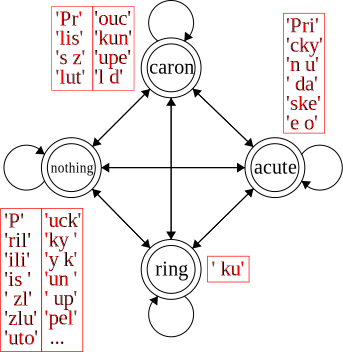
\includegraphics{automata.pdf}
        \caption{3-gram based Hidden Markov Model emitting Czech sentence
        \textit{P\v{r}\'{i}li\v{s} \v{z}lu\v{t}ou\v{c}k\'{y}  k\r{u}\v{n} \'up\v{e}l \v{d}\'{a}belsk\'{e} {\'{o}dy.}}
        (\textit{Possible observations} are placed in a red box counter clockwise from their respective HMM \textit{states})}

        \label{fig:auto}
    \end{figure*}
    The training data sets come from localizations of Wikipedia (therefore having some language norms),
    testing sets may contain text from other websites too.
    Corpora were built for training the bidirectional character-level recurrent neural-network in~\cite{naplava},
    which is the current state-of-the-art. During the evaluation of this project, corpora are temporarily available on \url{http://herbert.saarland/corpora.zip}

    \section{Method}\label{sec:method}
    As decided in our final project assignment, we are going to use represent our problem using Hidden Markov Models,
    trained using the Baum-Welch algorithm for ML estimate.
    We will be finding the word diacritization using the Viterbi algorithm.

    We have dropped the idea of implementing a competitive Na\"{i}ve Bayes classifier in favor
    of training and testing our model on numerous languages.

    \subsection{Rejected approaches}\label{subsec:rejected-approaches}
    The original idea was to have the HMM hidden states represent all \textbf{possible diacriticisations} of
    the \textbf{entire words} in the observable sequence.
    This method turned out to be inefficient due to its space complexity and to the fact that the most of the
    words of the language are actually the ones we did not observe in training data (Zipf's Law).

    Having a \textbf{character-level} HMM, switching between the states denoting the diacritical marks turns to be
    vastly inaccurate\footnote{in fact, see the unigram model's results in table~\ref{tab:measures}}, as
    the most common diacritization of every character alone is usually one with no diacritics.
    Using the ML estimation, we then arrive to a costly way to output a text without diacritics.

    \subsection{Accepted approach}\label{subsec:accepted-approach}
    The final approach we chose to follow was to be observing the \textbf{n-grams} of characters as occured
    in training data, tagging every such a n-gram with a diacritical mark over its last character, as in \textbf{figure~\ref{fig:auto}}.

    This approach significantly reduces the complexity (as there is only a constant number of HMM states -- signs)
    while maintaining better accuracy which is rising with the $n$.



    \section{Implementation}\label{sec:implementation}
    For simplicity and performance optimization, we have decided to build the explained system as a wrapper
    of the \textsf{NLTK}'s \texttt{HiddenMarkovModelTagger} and \texttt{HiddenMarkovModelTrainer} classes~\cite{nltk}.
    Our legacy in-house made HMM can be found at (might still get used in future if there is an optimization we can
    use it for):

    \noindent\url{https://github.com/heruberuto/diacritic-restoration/blob/master/models/hmm.py}

    Class \texttt{HmmNgramRestorer} serves as the facade for the \textsf{NLTK}'s and offers additional (de)serialization
    using \textsf{Pickle}.
    Upon training, class \texttt{CorpusNgramBuffer} mimics the \texttt{list} \textsf{NLTK} is trying to
    iterate through, outputting a parsed tagged n-grams for each line of a buffered file, thus enabling training on collections that would not fit in memory.

    Class \texttt{DiacriticsAccuracyCounter} is instantiated during the HMM testing, collecting scores for the
    accuracy experiments.

    The core modules \texttt{accents.py} and \texttt{diacritics\_restorer.py} were documented in detail using
    standardized Sphinx docstrings.

    The scripts for detokenizing corpora, conducting experiments and generating outputs in \texttt{\{evaluate,detokenize\_corpora,evaluate,pretrain,measurement\_table\}.py}
    are documented in-line, sufficiently to their complexity.

    \begin{table}
        \begin{tabular}{|l|l|l||l|l|l|l|l|}
            \hline
            \multirow{2}{*}{\textbf{language}} & \textbf{training} & \textbf{diacritical} & \multirow{2}{*}{\textbf{$n$}} &\multicolumn{4}{c|}{\textbf{accuracy}} \\ \cline{5-8}
            & \textbf{sentences} & \textbf{words} & & \textbf{tag} & \textbf{word} & \textbf{dia-word} & \textbf{alpha-word} \\
            \hhline{|=|=|=#=|=|=|=|=|}
            \textbf{Croatian} & 802,610 & 14.3\% & 1 & 0.977 & 0.857 & 0 & 0.85\\ \cline{4-8}
            & & & 2 & 0.98 & 0.874 & 0.206 & 0.868\\ \cline{4-8}
            & & & 3 & 0.985 & 0.903 & 0.491 & 0.898\\ \cline{4-8}
            & & & 4 & \textbf{0.989} & \textbf{0.929} & \textbf{0.618} & \textbf{0.925}\\ \cline{4-8}
            \hline
            \textbf{Czech} & 952,909 & 47.8\% & 1 & 0.892 & 0.522 & 0 & 0.498\\ \cline{4-8}
            & & & 2 & 0.904 & 0.549 & 0.141 & 0.527\\ \cline{4-8}
            & & & 3 & 0.924 & 0.628 & 0.321 & 0.61\\ \cline{4-8}
            & & & 4 & \textbf{0.94} & \textbf{0.689} & \textbf{0.433} & \textbf{0.674}\\ \cline{4-8}
            \hline
            \textbf{Slovak} & 613,727 & 41.1\% & 1 & 0.922 & 0.589 & 0 & 0.564\\ \cline{4-8}
            & & & 2 & 0.925 & 0.614 & 0.123 & 0.591\\ \cline{4-8}
            & & & 3 & 0.938 & 0.669 & 0.274 & 0.65\\ \cline{4-8}
            & & & 4 & \textbf{0.951} & \textbf{0.727} & \textbf{0.42} & \textbf{0.71}\\ \cline{4-8}
            \hline
            \textbf{Irish} & 50,825 & 29.7\% & 1 & 0.942 & 0.703 & 0 & 0.695\\ \cline{4-8}
            & & & 2 & 0.948 & 0.732 & 0.21 & 0.725\\ \cline{4-8}
            & & & 3 & 0.957 & 0.778 & 0.403 & 0.772\\ \cline{4-8}
            & & & 4 & \textbf{0.961} & \textbf{0.8} & \textbf{0.447} & \textbf{0.795}\\ \cline{4-8}
            \hline
            \textbf{Hungarian} & 1,294,605 & 47.4\% & 1 & 0.906 & 0.526 & 0 & 0.507\\ \cline{4-8}
            & & & 2 & 0.906 & 0.52 & 0.0792 & 0.501\\ \cline{4-8}
            & & & 3 & 0.924 & 0.587 & 0.267 & 0.57\\ \cline{4-8}
            & & & 4 & \textbf{0.939} & \textbf{0.649} & \textbf{0.38} & \textbf{0.635}\\ \cline{4-8}
            \hline
            \textbf{Polish} & 1,069,841 & 31.6\% & 1 & 0.946 & 0.684 & 0 & 0.669\\ \cline{4-8}
            & & & 2 & 0.949 & 0.701 & 0.164 & 0.686\\ \cline{4-8}
            & & & 3 & 0.961 & 0.762 & 0.353 & 0.75\\ \cline{4-8}
            & & & 4 & \textbf{0.969} & \textbf{0.809} & \textbf{0.493} & \textbf{0.8}\\ \cline{4-8}
            \hline
            \textbf{Romanian} & 837,647 & 28.2\% & 1 & 0.95 & 0.723 & 0.0234 & 0.709\\ \cline{4-8}
            & & & 2 & 0.953 & 0.742 & 0.164 & 0.729\\ \cline{4-8}
            & & & 3 & 0.958 & 0.768 & 0.31 & 0.757\\ \cline{4-8}
            & & & 4 & \textbf{0.964} & \textbf{0.797} & \textbf{0.431} & \textbf{0.787}\\ \cline{4-8}
            \hline
            \textbf{French} & 1,818,618 & 16.6\% & 1 & 0.97 & 0.834 & 0 & 0.826\\ \cline{4-8}
            & & & 3 & 0.971 & 0.84 & 0.0933 & 0.833\\ \cline{4-8}
            & & & 4 & \textbf{0.975} & \textbf{0.861} & \textbf{0.274} & \textbf{0.854}\\ \cline{4-8}
            \hline
            \textbf{Spanish} & 1,735,516 & 11.8\% & 1 & 0.981 & 0.882 & 0 & 0.88\\ \cline{4-8}
            & & & 3 & 0.982 & 0.893 & 0.218 & 0.89\\ \cline{4-8}
            & & & 4 & \textbf{0.985} & \textbf{0.909} & \textbf{0.378} & \textbf{0.907}\\ \cline{4-8}
            \hline
            \textbf{Latvian} & 315,807 & 46.8\% & 1 & 0.915 & 0.532 & 0 & 0.502\\ \cline{4-8}
            & & & 3 & 0.924 & 0.589 & 0.24 & 0.563\\ \cline{4-8}
            & & & 4 & \textbf{0.939} & \textbf{0.654} & \textbf{0.38} & \textbf{0.632}\\ \cline{4-8}
            \hline
        \end{tabular}
        \caption{Measurements of per-tag (single diacritical mark) and per-word accuracy
        of an $n$-gram based HMM diacritic restorer.
        We call dia-word a word that contains at least one diacritical character.
        The dia-word percentage is listed for testing set.
        We call alpha-word a word with at least one alphabetic character.
        } \label{tab:measures}
    \end{table}
    \section{Measuring accuracy}\label{sec:measuring-accuracy}
    Please see the \textbf{table~\ref{tab:measures}} for the result of our measuring experiments.

    The measurement procedure can be found within class \texttt{DiacriticsAccuracyCounter} and can be instantiated running
    \texttt{evaluate.py}.

    \pagebreak
    \pagebreak
    We have measured 4 scores - the accuracy of tags (single diacritic character), the accuracy of words (at their entirety),
    accuracy of words with at least one diacritical mark, and the standard accuracy of alpha words (words with at least one alphabetic character).

    We have observed that the accuracy rises significantly with the size of $n$-grams and that some languages are significantly
    easier (harder) than the others (e.g.\ Croatian).

    That can be caused by a simplicity of diacritical rules and their disambiguity.
    Sadly, we could not conclude the experiments for our most accurate feasible models with $n=6$ due to
    running out of memory during the tests.



    \section{Demos}\label{sec:demos}
    Please see the attached demonstration sheet \texttt{demos.ipynb}, that covers all the basic
    functionalities of our system.

    It also presents several pre-trained models we consider enjoyable to play around with.


    \section{Conclusions}\label{sec:conclusions}
    As hard as we tried, the accuracy got nowhere near the current state-of-the-art systems.
    For example, our 4-gram Croatian model has an alpha-word accuracy of 92.5\%,
    properly trained \textit{Lexicon} model (that replaces every word with its most common observed diacritization)
    achieves 99.31\% and the N\'{a}plava's neural networks~(\cite{naplava}) get 99.67\%.
    \subsection{Recommendations}\label{subsec:recommendations}
    Throughout implementing and testing our models, we have made several remarks on the possible system improvements and further research motivations:
    \begin{itemize}
        \item \textbf{``Tailed''} n-grams -- the HMM state could not be the diacritical mark over n-gram's last letter, but, think, the penultimate one --- that would give the tagger some context from both sides and would further punish faults of ``deciding too early'' (tagging ``\ldots\v{c}hodit'' even when ``ch'' behaves as a single letter with no possible diacritizations in Czech --- and the trainings cover that)
        \item \textbf{Combine with Lexicon} -- the HMM tagger could work well deciding ambiguities (or unobserved words) for the Lexicon system, thus creating system more accurate than both the original ones (if such an ambiguity decisioning is not implemented in \textit{Lexicon} already as it is)
    \end{itemize}
    \newpage
    \bibliography{references}
    \bibliographystyle{plain}
\end{document}
